
\documentclass[11pt]{article}


\usepackage{a4wide}
\usepackage{graphicx}
\usepackage{listings}
\usepackage{xcolor}

\setlength{\parindent}{0pt}


\definecolor{codegreen}{rgb}{0,0.6,0}
\definecolor{codegray}{rgb}{0.5,0.5,0.5}
\definecolor{codepurple}{rgb}{0.58,0,0.82}
\definecolor{backcolour}{rgb}{0.95,0.95,0.92}

\lstset{
    basicstyle=\ttfamily,      % 设置基本字体
    breaklines=true,           % 自动换行
    backgroundcolor=\color{backcolour},   
    commentstyle=\color{codegreen},
    keywordstyle=\color{magenta},
    numberstyle=\tiny\color{codegray},
    stringstyle=\color{codepurple},
    basicstyle=\ttfamily\footnotesize,
    breakatwhitespace=false,         
    breaklines=true,                 
    captionpos=b,                    
    keepspaces=true,                 
    numbers=left,                    
    numbersep=5pt,                  
    showspaces=false,                
    showstringspaces=false,
    showtabs=false,                  
    tabsize=2
}

\begin{document}

\title{Pentesting Report: Smart WiFi Camera}
\author{Haohan Fu (), Jiayang Xu (2829543), Zhengyang Cheng (),
    \\ Xi Wang (), Xibin Yu () and Haoyu Ju ()}
\date{12, March, 2025}
\maketitle

\section{Executive summary}

Give the high lights of your report, what are your key results and
recommendations?

\section{High-level description of the device}

What is the device and what does it do? How does it work? Does it take
commands, from a phone app? A cloud server? How does the user set it up? Etc.

The Goowls smart home camera, shown in figure 1:
\begin{figure}[htbp]
    \centering
    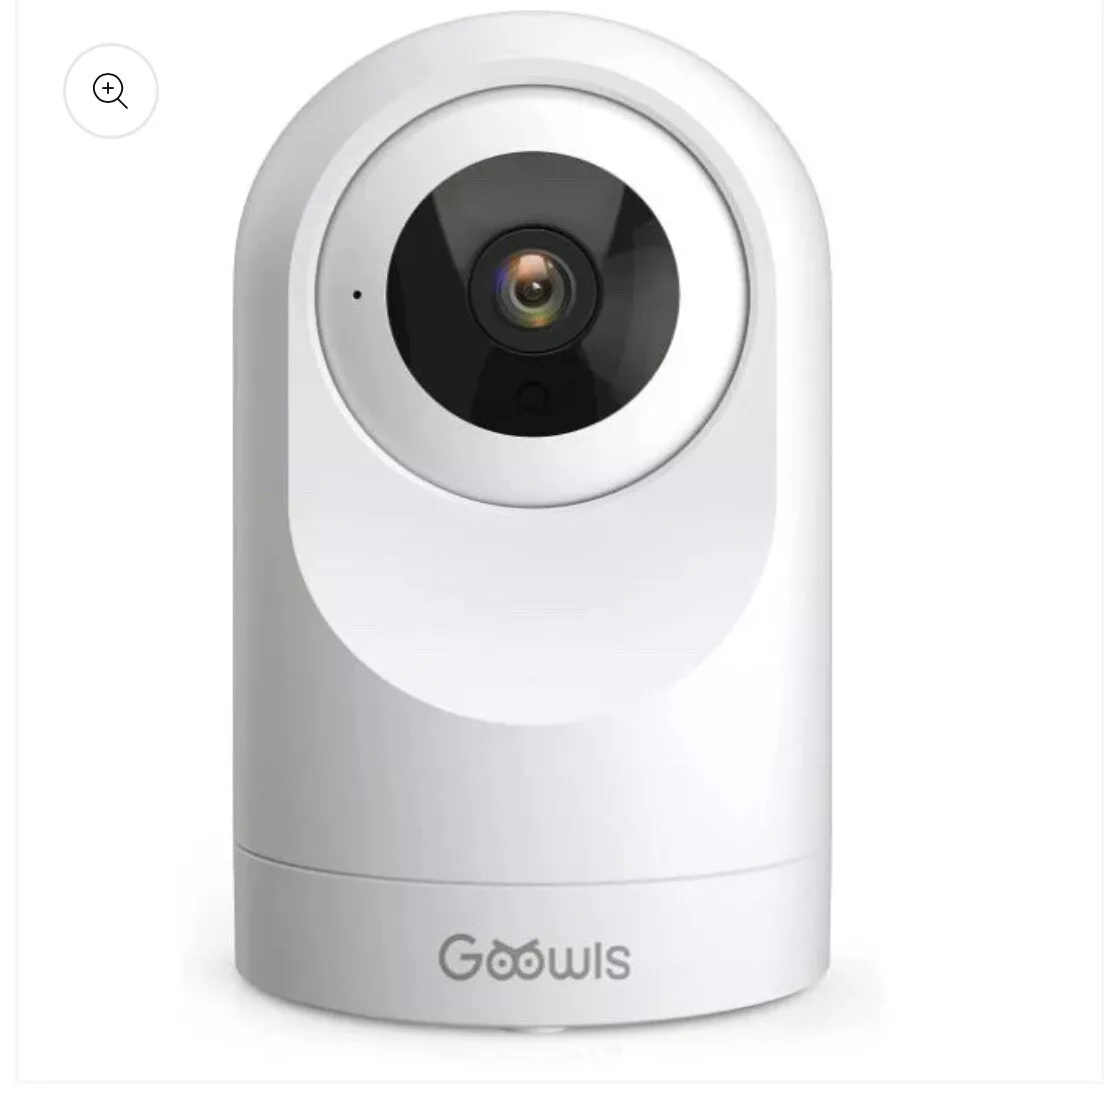
\includegraphics[width=0.5\textwidth]{imgs/camera.png}
    \caption{conponent of smart home camera}
\end{figure}

The Goowls Smart Home Camera is a versatile security device designed to enhance
home monitoring. Users can integrate multiple Goowls cameras into their smart
home ecosystem, allowing comprehensive surveillance across various areas of
their residence.

Central to this system is the camera itself, which offers 1080p high-definition
video quality for clear and detailed footage. Equipped with two-way audio, it
enables real-time communication between the user and individuals near the
camera. The device supports both local storage via a 4-64 GB Class 10 TF card
and cloud storage options, providing flexibility in video recording management.

To operate the Goowls camera, users need to download the YI IoT app, available
on both the Apple App Store and Google Play Store. Once installed and
configured, the app allows users to view live video feeds, replay recorded
footage, and receive motion detection alerts. Additionally, users can assign
specific names to each camera's location (e.g., "Living Room" or "Nursery") for
organized monitoring.

The Goowls camera is compatible with Amazon Alexa, enabling voice-controlled
access to live feeds. To set up this feature, users must add the YI IoT skill
to their Alexa app and link their account. Once connected, voice commands can
be used to display camera feeds on Alexa-enabled devices.

\section{Investigating the device}

\subsection{Analysing the device setup}

Describe the technical details of how the device is set up by the user. What
protocols are used and how? How did you fine this out? Give technical details,
and enough information to ensure that your analysis is repeatable by someone
else.

\subsection{Analysing the device in use}

Describe the technical details of how the device is used after set up. What
protocols are used and how? How did you fine this out. Give technical details,
and enough information to ensure that your analysis is repeatable by someone
else.

\subsection{Analysing the apk file}

To further analyse the app, the app was decompiled by first downloading the apk file (via Google Play) and then using dex2jar and jadx-gui to decompile the apk. \par
This process was able to retrieve most of the classes used by the app, and this code was then analysed to check for possible vulnerabilities in the app. \par
Because the code base of the app was so large, we focused and searched for specific keywords, which was more efficient and useful than going through the entire code. The keywords used were as follows:

\begin{itemize}
    %\item connect, server, ip address, port - for connection details
    %\item UID, username, password - for authentication details
    \item encryption, key, RSA, AES, SHA, ciphersuite - for details related to the security aspect of the app
\end{itemize}

There following are the interesting results from these findings :

\begin{enumerate}
    \item AES \par
    It shows that it use AES-CBC as encryption method.

          \begin{lstlisting}[language=Java, caption=com.ants360.yicamera.base.p.java]
public final Cipher d(boolean retry) throws Exception {
    Key b10 = b();
    Cipher cipher = Cipher.getInstance("AES/CBC/PKCS7Padding");
    try {
        cipher.init(3, b10);
    } catch (KeyPermanentlyInvalidatedException e10) {
        this.f9903a.deleteEntry(f9897b);
        if (!retry) {
            throw new Exception("Could not create the cipher for fingerprint authentication.", e10);
        }
        d(false);
    }
    return cipher;
}
\end{lstlisting}

    \item RSA \par
    It shows that it generate key pair for RSA.

          \begin{lstlisting}[language=Java, caption=v4.c.java]
public static final PublicKey c(@k String key) {
    e0.p(key, "key");
    byte[] decode = Base64.decode(u.l2(u.l2(u.l2(key, "\n", "", false, 4, null), "-----BEGIN PUBLIC KEY-----", "", false, 4, null), "-----END PUBLIC KEY-----", "", false, 4, null), 0);
    e0.o(decode, "decode(pubKeyString, Base64.DEFAULT)");
    PublicKey generatePublic = KeyFactory.getInstance("RSA").generatePublic(new X509EncodedKeySpec(decode));
    e0.o(generatePublic, "kf.generatePublic(x509publicKey)");
}
\end{lstlisting}

    \item SHA-256 \par
    It shows that it uses SHA-256 as hashing algorithm.

          \begin{lstlisting}[language=Java, caption=com.xiaoyi.base.util.y.java]
public final byte[] d(String key) {
    byte[] bytes = "gcQu4mcDjQkPjcX1YY2X6xNaWyiWF0dD".getBytes();
    try {
        MessageDigest messageDigest = MessageDigest.getInstance("SHA-256");
        messageDigest.reset();
        return messageDigest.digest(key.getBytes("UTF-8"));
    } catch (UnsupportedEncodingException e10) {
        e10.printStackTrace();
        return bytes;
    } catch (NoSuchAlgorithmException e11) {
        e11.printStackTrace();
        return bytes;
    }
}
\end{lstlisting}
\end{enumerate}

\section{Possible attacks against the device}

\subsection{Attacks by a local attacker with wi-fi access}

For an attacker with wifi access, he can use burp to conduct a man-in-the-middle attack when the user's mobile phone already has a forged certificate installed. When the device sends data to the server, its packets will be intercepted by burp, if the certificate is successfully installed, then the browser will not have a security alert, on the contrary, it will warn the user that the connection is not private, as shown in Figure \ref{Connection is not private}. When the packet is intercepted, the contents can be tampered with by burp and sent to the server, and the server's response message can also be intercepted by burp, so that the man-in-the-middle attack is fully realised.\par

\begin{figure}[h]
    \centering
    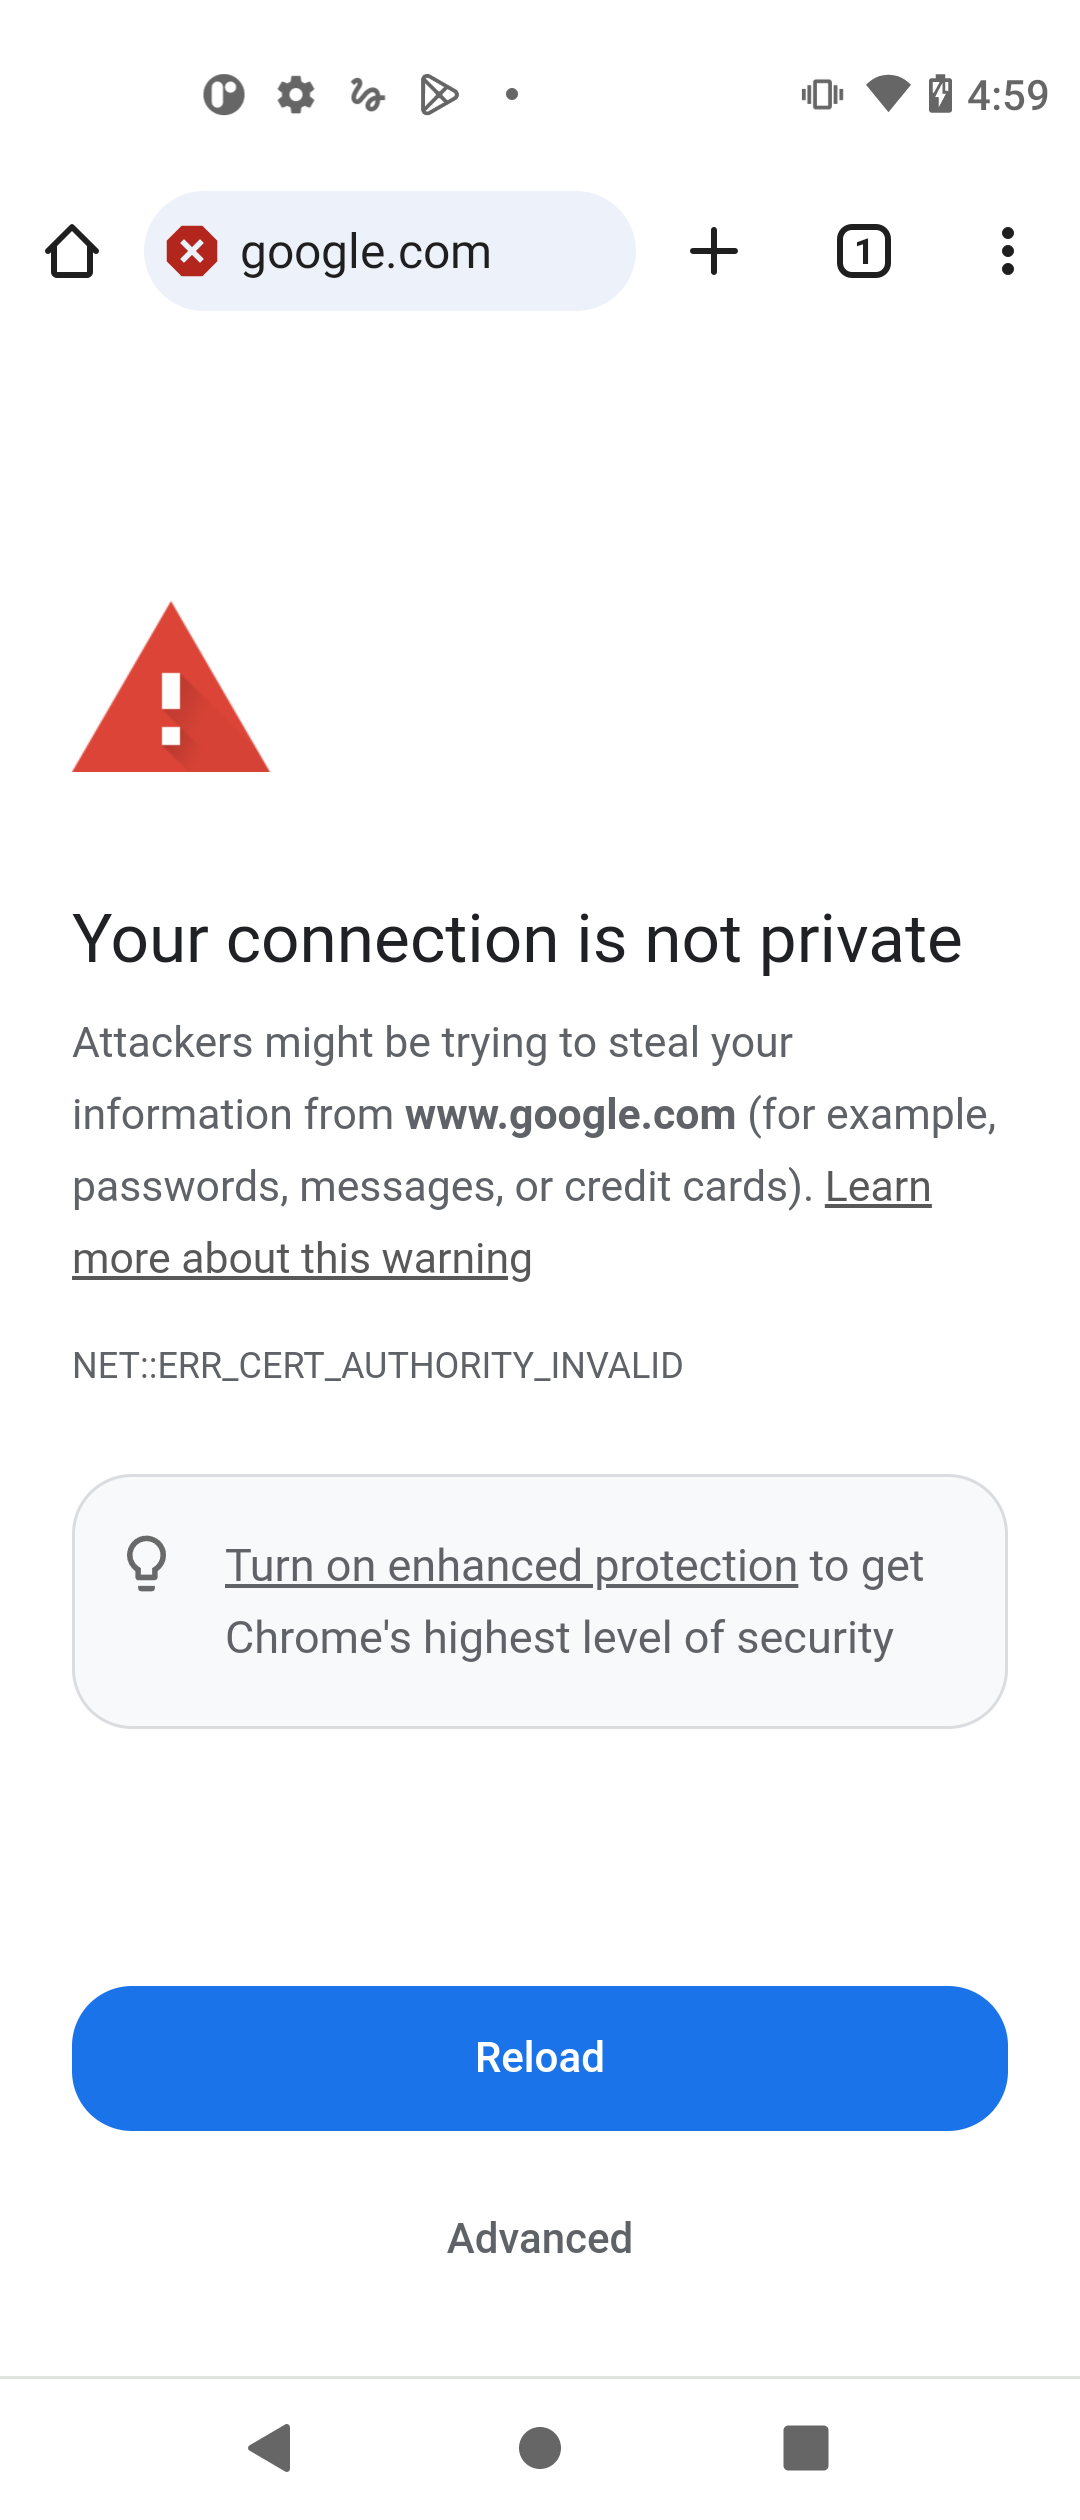
\includegraphics[width=0.3\textwidth]{imgs/MITM.png}
    \caption{Connection is not private}
    \label{Connection is not private}
\end{figure}

We carried out the man-in-the-middle attack by modifying the username in the app. In our man-in-the-middle attack on the device, we found that every time a request is sent, the message generated by the client carries a message authentication code, and when the message is tampered with, the server will fail to authenticate and reject the request, and then force the client to log out. \par
Since the message authentication code is generated based on the content of the packet, we believe that we can carry out a replay attack, will have intercepted the successful access to the packet to save, and in the user to modify the packet sent to the server again using burp, the results of the verification of the re-sent packet is valid, the user unknowingly by us to modify the data on the server side. As shown in the Figure 3\ref{Burp}, we have used burp to intercept the packet in which the user changed his username to 0066. After the user changed his username to something else (e.g. 01), we re-sent the packet to the server to change his username to 0066, and as shown in Figure \ref{Name changed} that after the user logged in again, his username has changed to 00, which proves that we have successfully carried out the man-in-the-middle attack.

\begin{figure}[htbp]
    \centering
    \begin{minipage}[b]{0.49\textwidth}
      \centering
      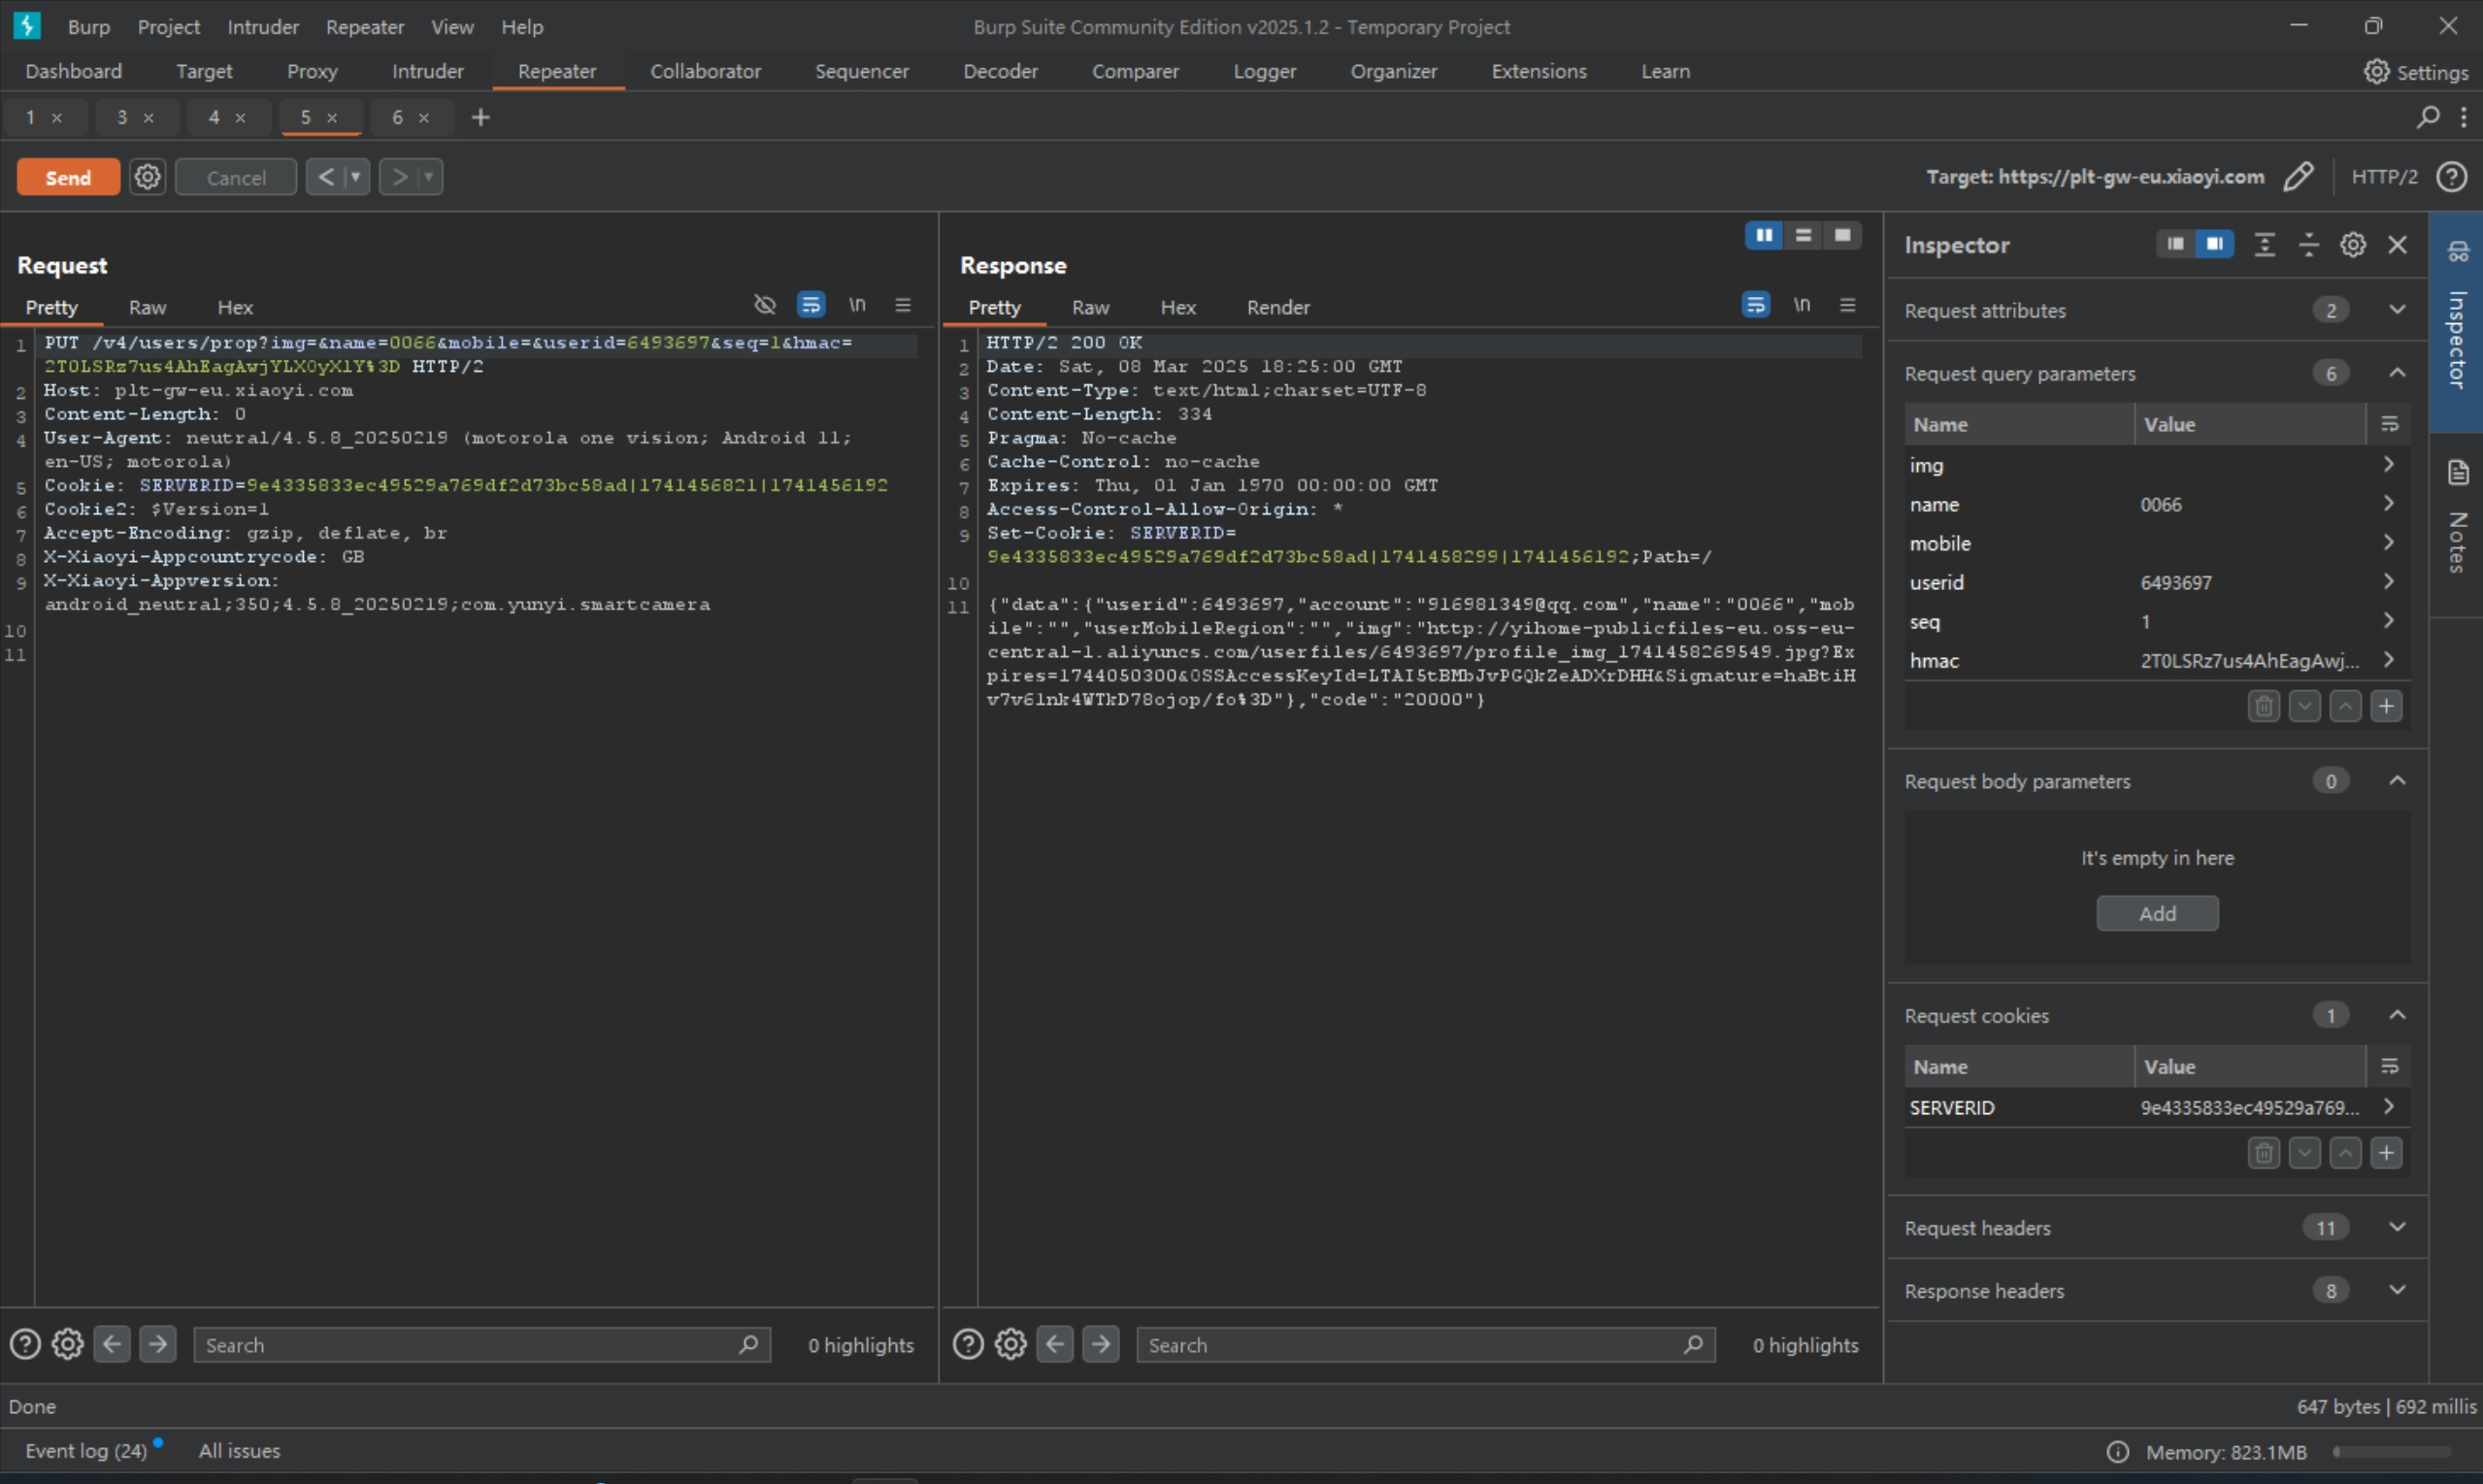
\includegraphics[width=1\textwidth]{imgs/BURP.png}
      \caption{Burp}
      \label{Burp}
    \end{minipage}
    \hfill
    \begin{minipage}[b]{0.49\textwidth}
      \centering
      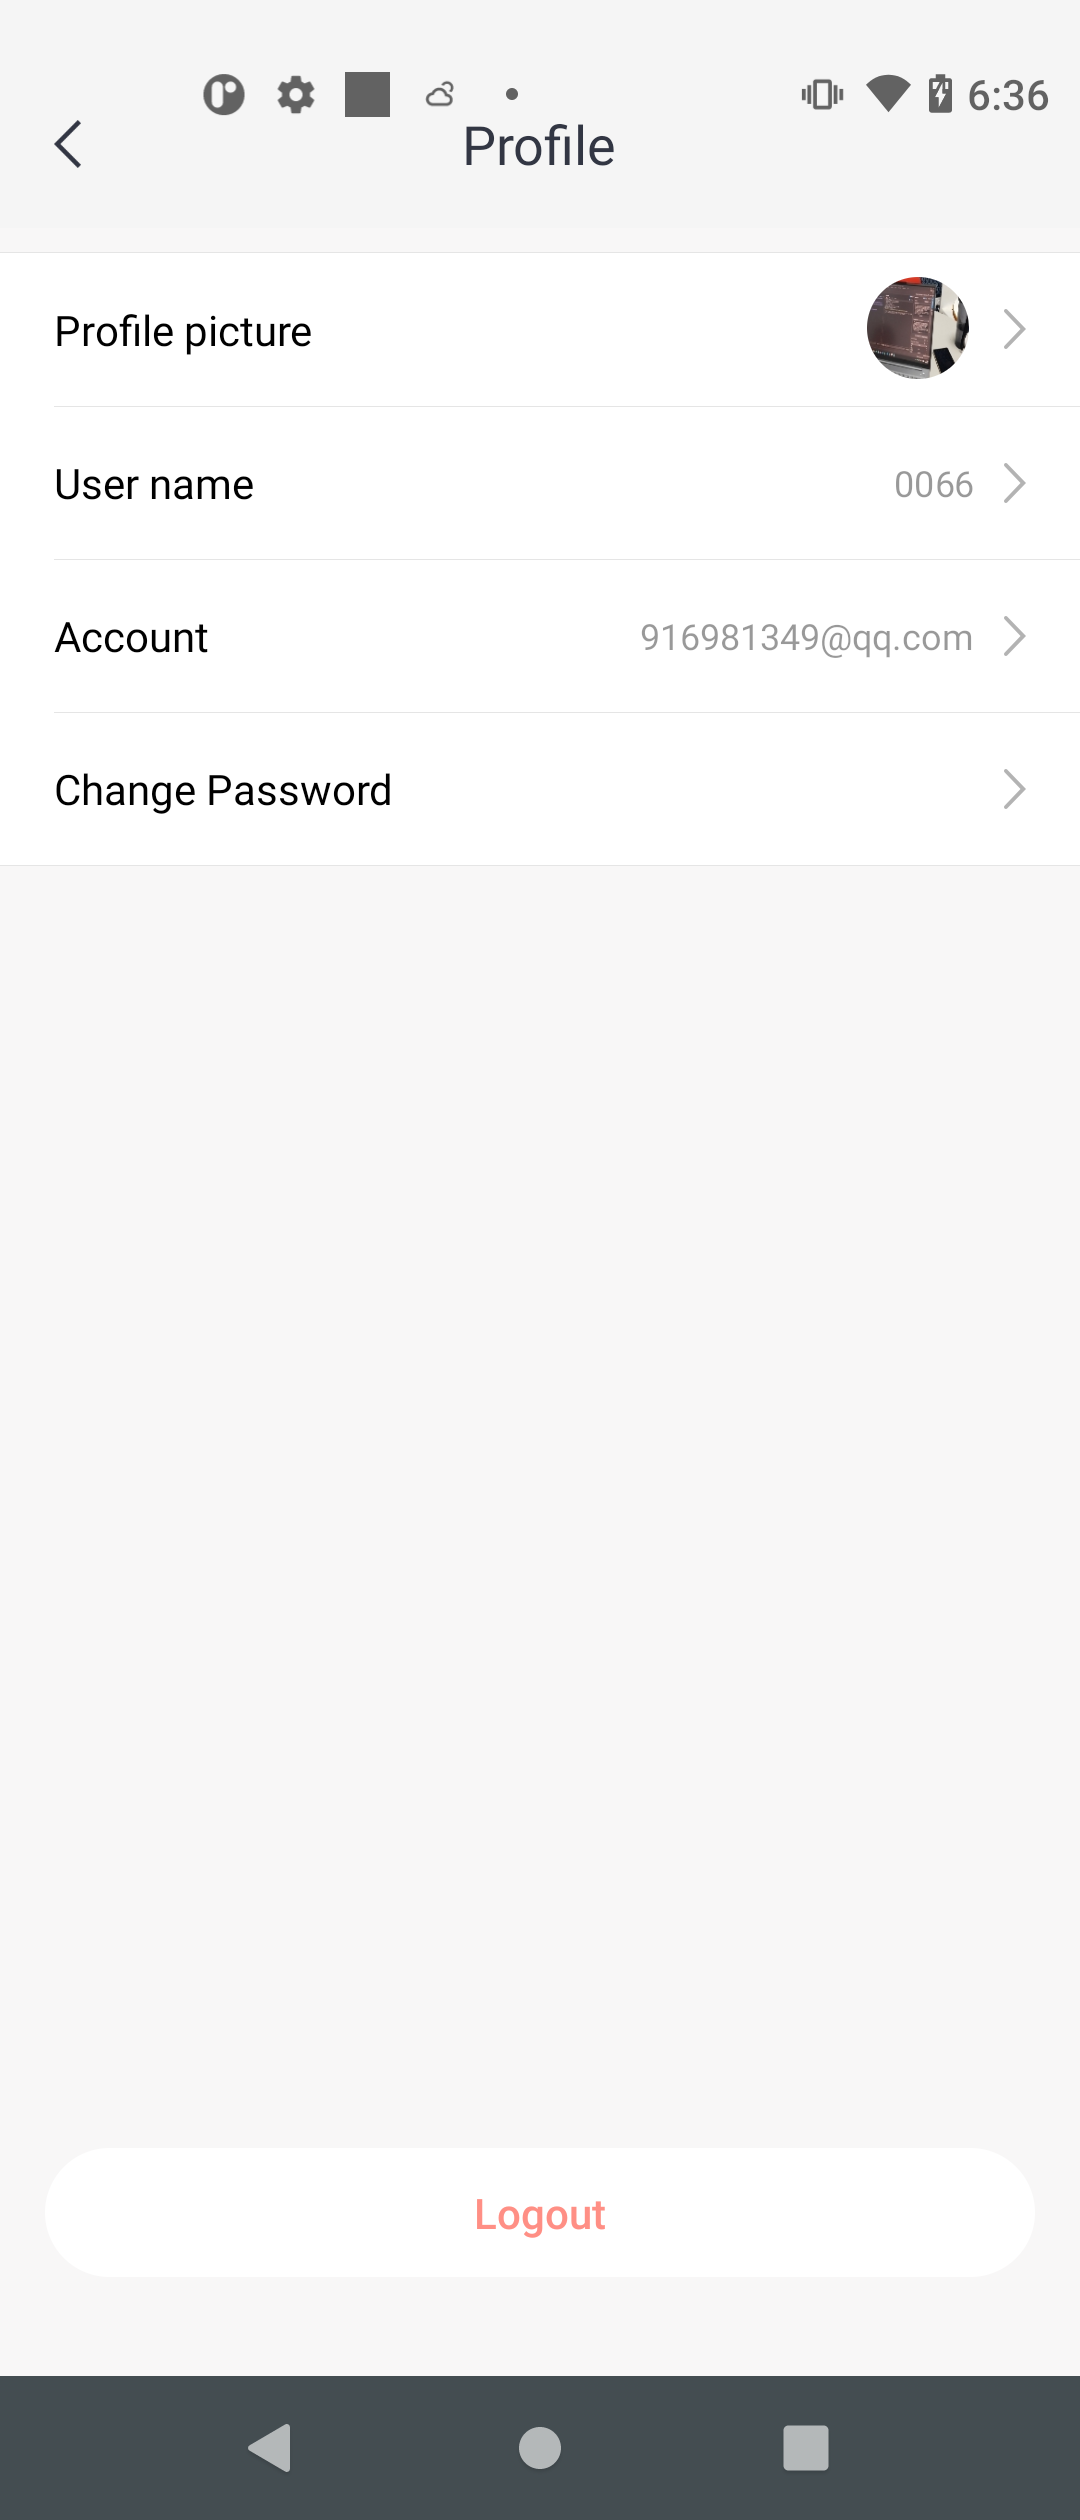
\includegraphics[width=0.5\textwidth]{imgs/name_changed.png}
      \caption{Name changed}
      \label{Name changed}
    \end{minipage}
  \end{figure}

\subsection{Attacks by a local attacker without wi-fi access}

Reset button

\subsection{Attacks by a remote attacker}

None

\section{Analysis of the weaknesses found}

MITM attack

Brute force attack

DDOS attack

\appendix

\section{Additional technical information}

Include additional technical information to support your report. APK files,
pcap files, Burp logs, a proof of concept attack code can be given to me on a
USB stick.
\end{document}

